\documentclass[a4paper,12pt]{article}
\addtolength{\oddsidemargin}{-1.cm}
\addtolength{\textwidth}{2cm}
\addtolength{\topmargin}{-3cm}
\addtolength{\textheight}{3.5cm}
\makeindex


\usepackage[pdftex]{graphicx}
\usepackage{makeidx}
\usepackage{float}
\usepackage{hyperref}
\hypersetup{
	colorlinks=true,
	linkcolor=blue,
	filecolor=magenta,      
	urlcolor=cyan,
}



% define the title
\author{CodeBlox}
\title{Tender}
\begin{document}
	\setlength{\parskip}{6pt}
	
	% generates the title
	\begin{titlepage}
		\begin{center}
			
\includegraphics[width=1\textwidth]{./Pictures/up_logo.png}\\[1.5cm] 
			\textsc{\LARGE Department of Computer Science} \\ [.5cm]
			\textsc{\Large Functional and Architectural Requirements} \\ [.5cm]
			\line(1,0){450}\\[.5cm]
			\huge{\bfseries Client: Gavin Potgieter}\\
			\line(1,0){450}\\[.5cm]
			\textsc{\LARGE Team: CodeBlox}\\ [0.5cm]
			
			
			\textsc{\large Tshepo Malesela (Bsc: Computer Science)}\\
			\textsc{\large Lethabo Mogase (Bsc: Computer Science)}\\
			\textsc{\large Lorenzo Spazzoli (Bsc: Computer Science)}\\
			\textsc{\large Bilal Muhammad (BIS: Multimedia)}\\
			\textsc{\large Dirk de Klerk (BIS: Multimedia)}\\ [3.9cm]
			
			\large\today
		\end{center}
	\end{titlepage}
	
	\tableofcontents
	\thispagestyle{empty}
	\footnotesize
	\normalsize
	
	
	
	
	\newpage
	\section{Introduction}
	The purpose of this document is to provide a detailed overview of the functional and architectural requirements with regard to the DropOff Project that was assigned to team CodeBlox. The document will be under constant revision, and will change as the project progresses. 
	
	{\noindent}It will provide the development team with a reference that can be used to develope from, thus ensuring that all functional and architectural requirements are met.
	
	{\noindent}The document will also serve as means of communication between the client and development team. Thus any additional requirements from the clients' side can be appended to the document, and has to be adhered to from the development side.
	
	\section{Project Objectives} The \textbf{primary objective} of the project is to create an automated service system that will provide customers with the ability to grant delivery personnel access to a drop safe and/or demarcated area of their home. This will ensure that deliveries to be made can be completed without the need of someone being physically present on the premises.
	
	{\noindent}Initially this will consist of the generation of a One Time Pin (OTP), that will be sent to the delivery personnel, granting them single access to the demarcated area. Once the delivery has been made. The user needs to be able to ensure that the residence is secure.
	
	{\noindent}If time allows it. The system will be expanded to use audio and video communication to validate the identity of the delivery person.
	
	{\noindent}In addition to the functionality of the system, it needs to be as \textbf{cost effective} as possible. This will allow a larger audience to gain access to the system. 
	
	{\noindent}The \textbf{secondary objective} (if time permits) is to make the system scalable. This will enable services to expand to other areas of the home. Thus allowing users an affordable solution to home automation.
	
	\newpage
	\section{Functional Requirements}
	
	\subsection{Users}
	The users module will be responsible for maintaining user information. Particularly it will specify what type of user it is. The module will also have the responsibility of storing demographic information about the users.
	
	\subsubsection{Scope}
	The scope of the Users module is shown below
	
	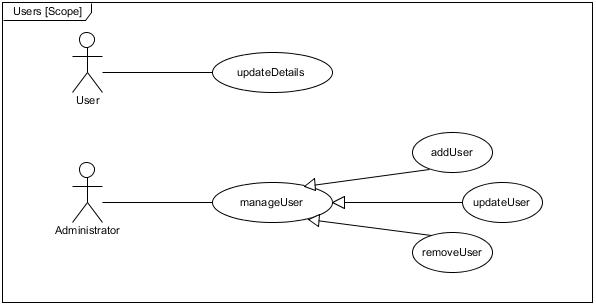
\includegraphics[width=1\textwidth]{./Pictures/UML/usersScope.jpg}\\[1.5cm]
	
	{\noindent}The scope of the Users module includes
	\begin{itemize}
		\item adding, removing, and modifying users on the system
		\item changing user information
	\end{itemize}
	
	\subsubsection{Domain Model}
	The domain model for the Users module is shown below
	
	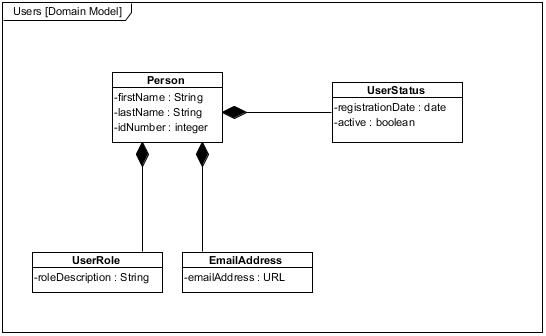
\includegraphics[width=1\textwidth]{./Pictures/UML/usersDomainModel.jpg}\\[1.5cm]	

	{\noindent}Each user has a firstname and a lastname, as well as an id number. The person will also have an email address associated with them that will be used for login purposes. Each person will also be associated with a role that will indicate if it is an administrator or general user. Lastly a status will be designated to each user to determine if they are active or not.	
	 
	\newpage
	\subsubsection{Use Cases}
	
	\begin{itemize}
		\item \textbf{addUser} - Allows an administrator to add a user to the system.\\[0.5cm]
		\textit{preconditions:}
			\begin{itemize}
				\item user does not already exist on the system
				\item creator possesses the role of administrator
			\end{itemize}
			
		\textit{postconditions:}
			\begin{itemize}
				\item a user is created.
				\item the user is added to the system.\\[0.5cm]
			\end{itemize}
			
		\item \textbf{removeUser} - Allows an administrator to remove a user to the system.\\[0.5cm]
		\textit{preconditions:}
			\begin{itemize}
				\item the user exists on the system
				\item remover possesses the role of administrator
			\end{itemize}
		
		\textit{postconditions:}
			\begin{itemize}
				\item a user is removed.
				\item the user is removed from the system.\\[0.5cm]
			\end{itemize}
			
		\item \textbf{updateUser} - Allows an administrator to modify a user on the system.\\[0.5cm]
		\textit{preconditions:}
			\begin{itemize}
				\item the user exists on the system
				\item modifier possesses the role of administrator
			\end{itemize}
		
		\textit{postconditions:}
			\begin{itemize}
				\item a users information is modified.\\[0.5cm]
			\end{itemize}
			
		\item \textbf{updateDetails} - Allows a general user to update their information.\\[0.5cm]
		\textit{preconditions:}
			\begin{itemize}
				\item the user exists on the system
				\item the user has to correct credentials
			\end{itemize}
		
		\textit{postconditions:}
			\begin{itemize}
				\item a users information is modified.
			\end{itemize}
	\end{itemize}
	
	\newpage
	\subsection{Controller}
	The controller module will be responsible for maintaining system status information as well as provide the user with system functionality. Particularly it will specify the current status of the drop box/area and allow the user to change this status through specific functions. This module will also be responsible for generating the OTP.
	
	\subsubsection{Scope}
	The scope of the Controller module is shown below
	
	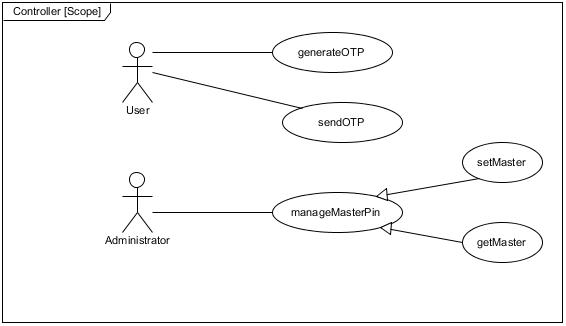
\includegraphics[width=1\textwidth]{./Pictures/UML/controllerScope.jpg}\\[1.5cm]
	
	{\noindent}The scope of the Users module includes
	\begin{itemize}
		\item generating, and sending an OTP.
		\item setting and getting a master OTP.
	\end{itemize}
	
	\newpage
	\subsubsection{Domain Model}
	The domain model for the Controller module is shown below
	
	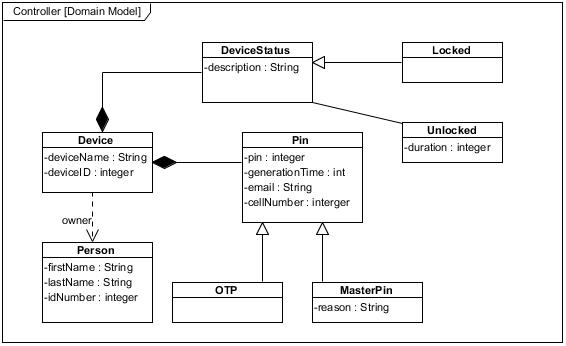
\includegraphics[width=1\textwidth]{./Pictures/UML/controllerDomainModel.jpg}\\[1.5cm]	
	
	{\noindent}Each user has a firstname and a lastname, as well as an id number. The person will also have an email address associated with them that will be used for login purposes. Each person will also be associated with a role that will indicate if it is an administrator or general user. Lastly a status will be designated to each user to determine if they are active or not.	
	
	\newpage
	\subsubsection{Use Cases}
	
	\begin{itemize}
		\item \textbf{addUser} - Allows an administrator to add a user to the system.\\[0.5cm]
		\textit{preconditions:}
		\begin{itemize}
			\item user does not already exist on the system
			\item creator possesses the role of administrator
		\end{itemize}
		
		\textit{postconditions:}
		\begin{itemize}
			\item a user is created.
			\item the user is added to the system.\\[0.5cm]
		\end{itemize}
		
		\item \textbf{removeUser} - Allows an administrator to remove a user to the system.\\[0.5cm]
		\textit{preconditions:}
		\begin{itemize}
			\item the user exists on the system
			\item remover possesses the role of administrator
		\end{itemize}
		
		\textit{postconditions:}
		\begin{itemize}
			\item a user is removed.
			\item the user is removed from the system.\\[0.5cm]
		\end{itemize}
		
		\item \textbf{updateUser} - Allows an administrator to modify a user on the system.\\[0.5cm]
		\textit{preconditions:}
		\begin{itemize}
			\item the user exists on the system
			\item modifier possesses the role of administrator
		\end{itemize}
		
		\textit{postconditions:}
		\begin{itemize}
			\item a users information is modified.\\[0.5cm]
		\end{itemize}
		
		\item \textbf{updateDetails} - Allows a general user to update their information.\\[0.5cm]
		\textit{preconditions:}
		\begin{itemize}
			\item the user exists on the system
			\item the user has to correct credentials
		\end{itemize}
		
		\textit{postconditions:}
		\begin{itemize}
			\item a user information is modified.
		\end{itemize}
	\end{itemize}
	 
	 
\end{document}
